\documentclass[main]{subfiles}
\begin{document}

\chapter{Switcheo Manual/Automático}

\section{Introducción}

Se pretende lograr que el sistema implementado pueda ser comandado de forma tanto manual como automática, buscándose además que la transición entre las dos formas de comando pueda realizarse en forma remota.\\
\\
Para ello, entonces, es necesario encontrar una forma de indicar al sistema que tipo de comando se desea utilizar. Se cuenta con un control remoto considerablemente complejo que, además, está diseñado para comandar una gran variedad de vehiculos radiocontrolados. Por este motivo, el control envía y recibe señales que no son utilizadas por el cuadricóptero. Es así, entonces, que se opta por reutilizar alguna de dichas señales para lograr el switcheo manual/automático.

\section{Señales del control remoto}

El sistema de transmisor/receptor que utiliza el control remoto (Walkera WK-2801 PRO) transmite la información a través de 8 canales mediante modulación PPM (pulse position modulation).\\
\\
En dicho esquema de modulación se parte de un frame temporal de duración fija que es dividido en $N$ partes iguales. Dichas partes son luego llevadas a 0 o Vcc para codificar así la información. Se trata, entonces, de un sistema de codificación temporal.\\

\section{Señal elegida}
Luego de un estudio detallado del transmisor y el receptor, pudo determinarse que la señal que se envía a través del canal etiquetado como GEAR no es utilizada en el comando del cuadricóptero. De igual manera, dicha señal es afectada únicamente por una llave existente en el control remoto. Dicha llave sólamente afecta a la señal presente en el canal GEAR, dejando invariantes el resto de las señales enviadas.\\
\\
La señal GEAR entonces verifica:

\begin{itemize}
\item Es comandada por un único elemento del control remoto
\item El elemento que la comanda no afecta ninguna otra señal
\item El control de cuadricóptero no utiliza dicha señal
\end{itemize}

En la figura \ref{fig:receptor} se indica el canal por el cual se transmite la señal GEAR. Cada canal es transmitido a través de 3 conductores, donde dos de ellos proveen voltajes de referencia Vcc (4.8V) y tierra (0V), mientras que el tercero es usado para transmitir la señal PPM.\\

\begin{figure}[H]
\begin{center}
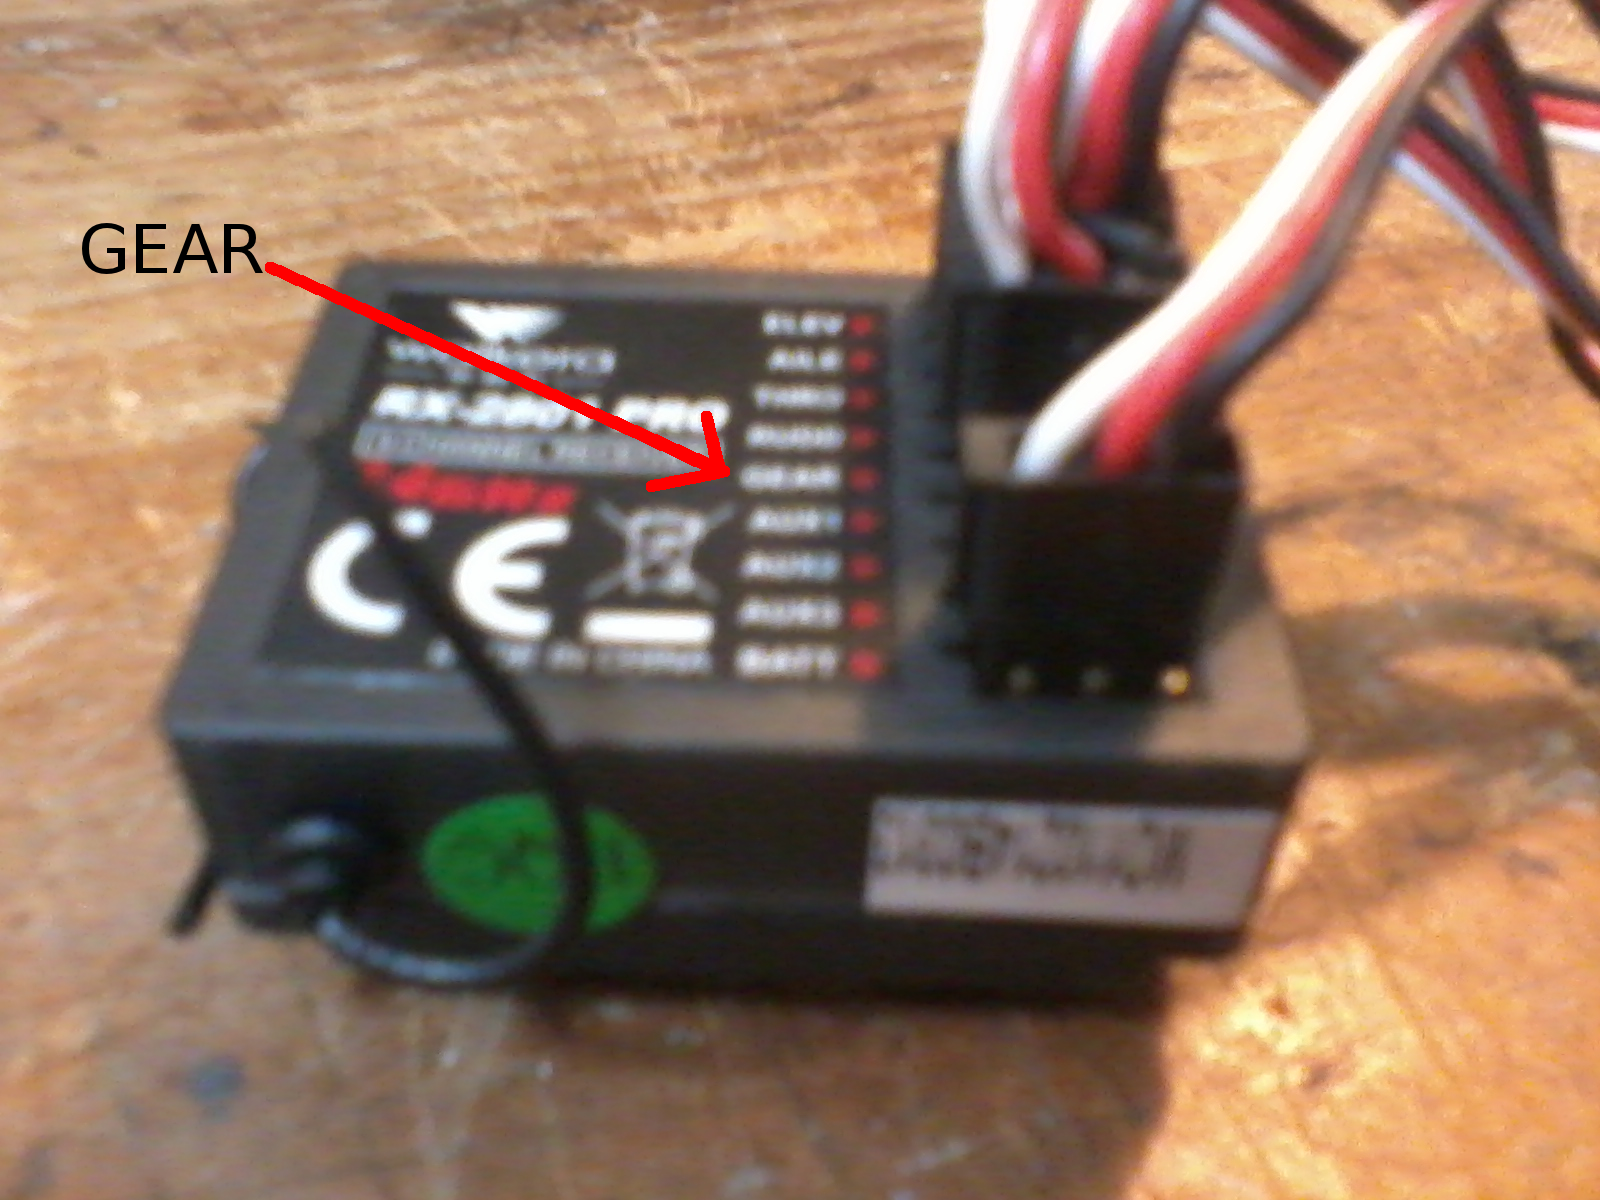
\includegraphics[width=0.7\textwidth]{./pics_switcheo/receptor.png}
\caption{Receptor}
\label{fig:receptor}
\end{center}
\end{figure}

Los conductores pueden ser identificados por su color según la siguiente tabla:\\

\begin{tabular}{|l|l|l|}
\hline
Color 		& Señal			&Tensión	\\
\hline
Negro		& Tierra		& 0V		\\
\hline
Naranja 	& Vcc			& 4.8V 		\\
\hline
Blanco 		& Datos(PPM) 	& 0V-4.8V 	\\
\hline
\end{tabular}
\\

En cuanto al control remoto, la señal del canal GEAR puede ser modificada mediante la llave indicada como GEAR SW en la figura \ref{fig:control}

\begin{figure}[H]
\begin{center}
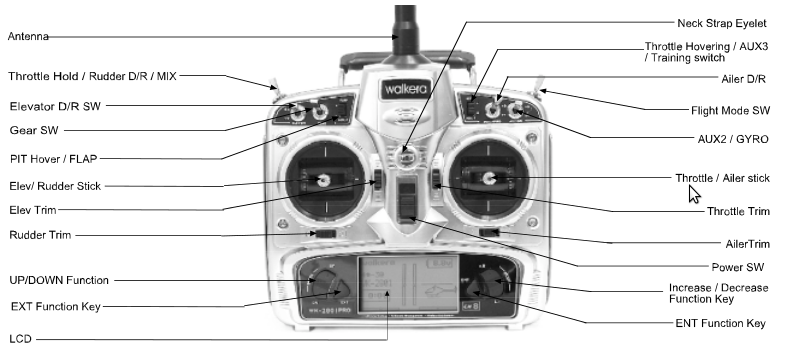
\includegraphics[width=0.7\textwidth]{./pics_switcheo/control.png}
\caption{Control remoto}
\label{fig:control}
\end{center}
\end{figure}

\section{Análisis de la señal}

Se procedió a estudiar la señal seleccionada mediante la adquisición de la misma con un osciloscópio. Pudo verse que cuando la llave GEAR SW está ``abajo'' la señal observada es una onda cuadrada (Tierra-Vcc) de frecuencia $f=52.41Hz$ y ciclo de trabajo 5.25\%, mientras que al estar la llave ``arriba'' el ciclo de trabajo varía, siendo este ahora 9.50\%.\\
\\
Es claro que lo que verdaderamente está sucediendo es que la posición de la llave baja se codifica seteando un cierto número de  frames temporales consecutivos a Vcc y dejando el resto de los frames a tierra, mientras que la posición alta se codifica seteando un mayor número de frames consecutivos a Vcc y dejando el resto a tierra.\\
\\
Lo expuesto anteriormente puede observarse en las figuras \ref{fig:GEAR_bajo} y \ref{fig:GEAR_alto}.

\begin{figure}[H]
\begin{center}
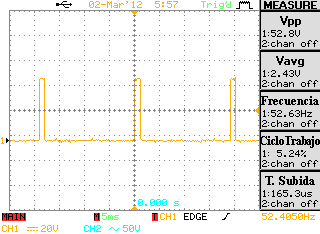
\includegraphics[width=0.7\textwidth]{./pics_switcheo/GEAR_bajo.png}
\caption{Señal con GEAR bajo}
\label{fig:GEAR_bajo}
\end{center}
\end{figure}

\begin{figure}[H]
\begin{center}
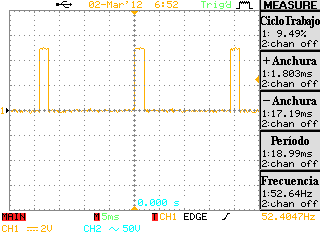
\includegraphics[width=0.7\textwidth]{./pics_switcheo/GEAR_alto.png}
\caption{Señal con GEAR alto}
\label{fig:GEAR_alto}
\end{center}
\end{figure}

También es posible observar la variación de la señal GEAR en el mismo control remoto, mediante la función MONITOR, tal como puede observarse en las figuras \ref{fig:control_bajo} y \ref{fig:control_alto}

\begin{figure}[H]
\begin{center}
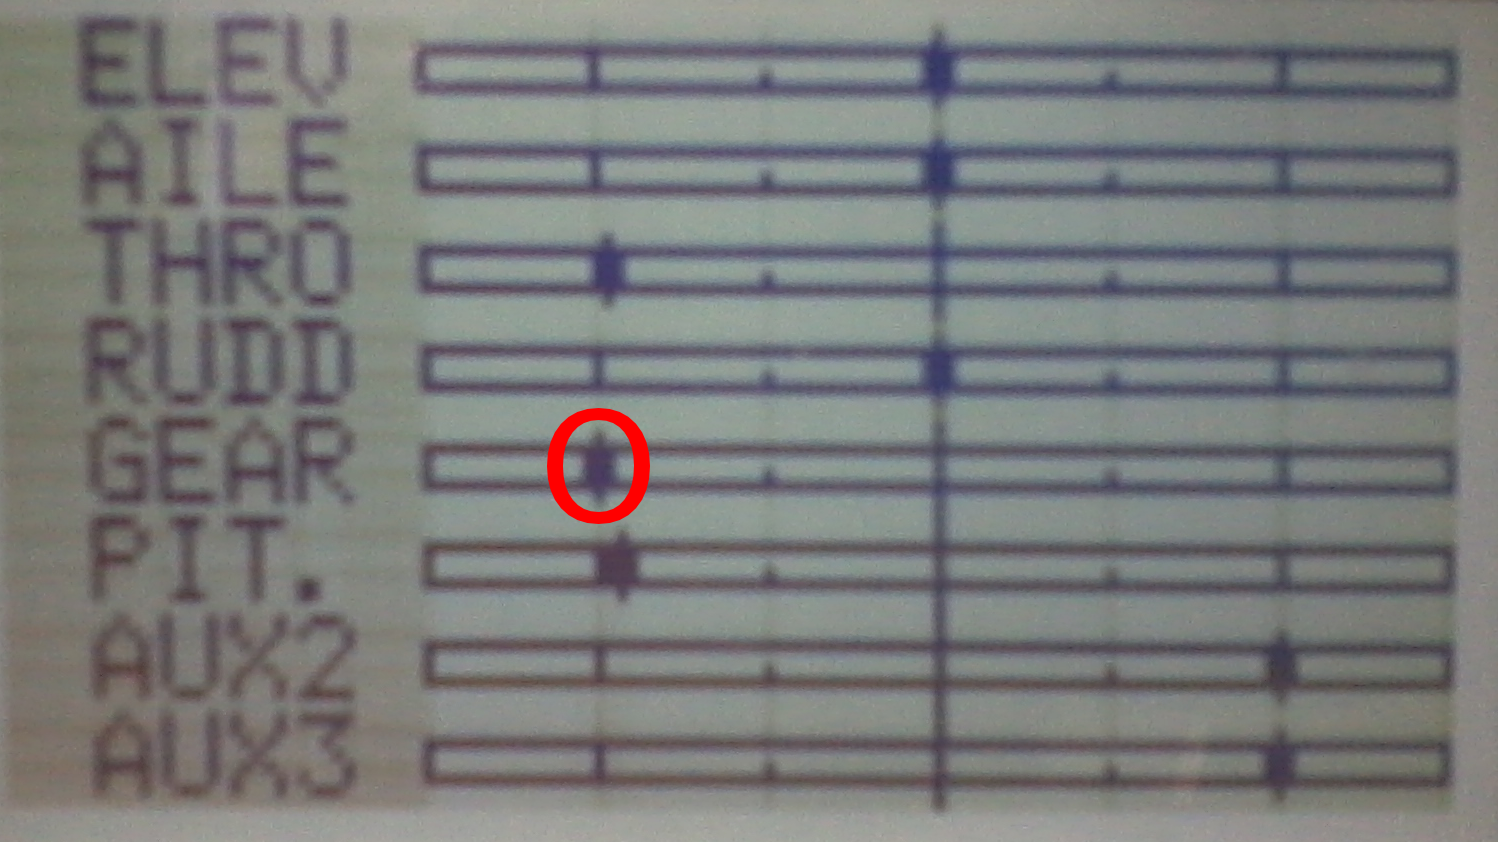
\includegraphics[width=0.7\textwidth]{./pics_switcheo/control_bajo.png}
\caption{Monitor con GEAR bajo}
\label{fig:control_bajo}
\end{center}
\end{figure}

\begin{figure}[H]
\begin{center}
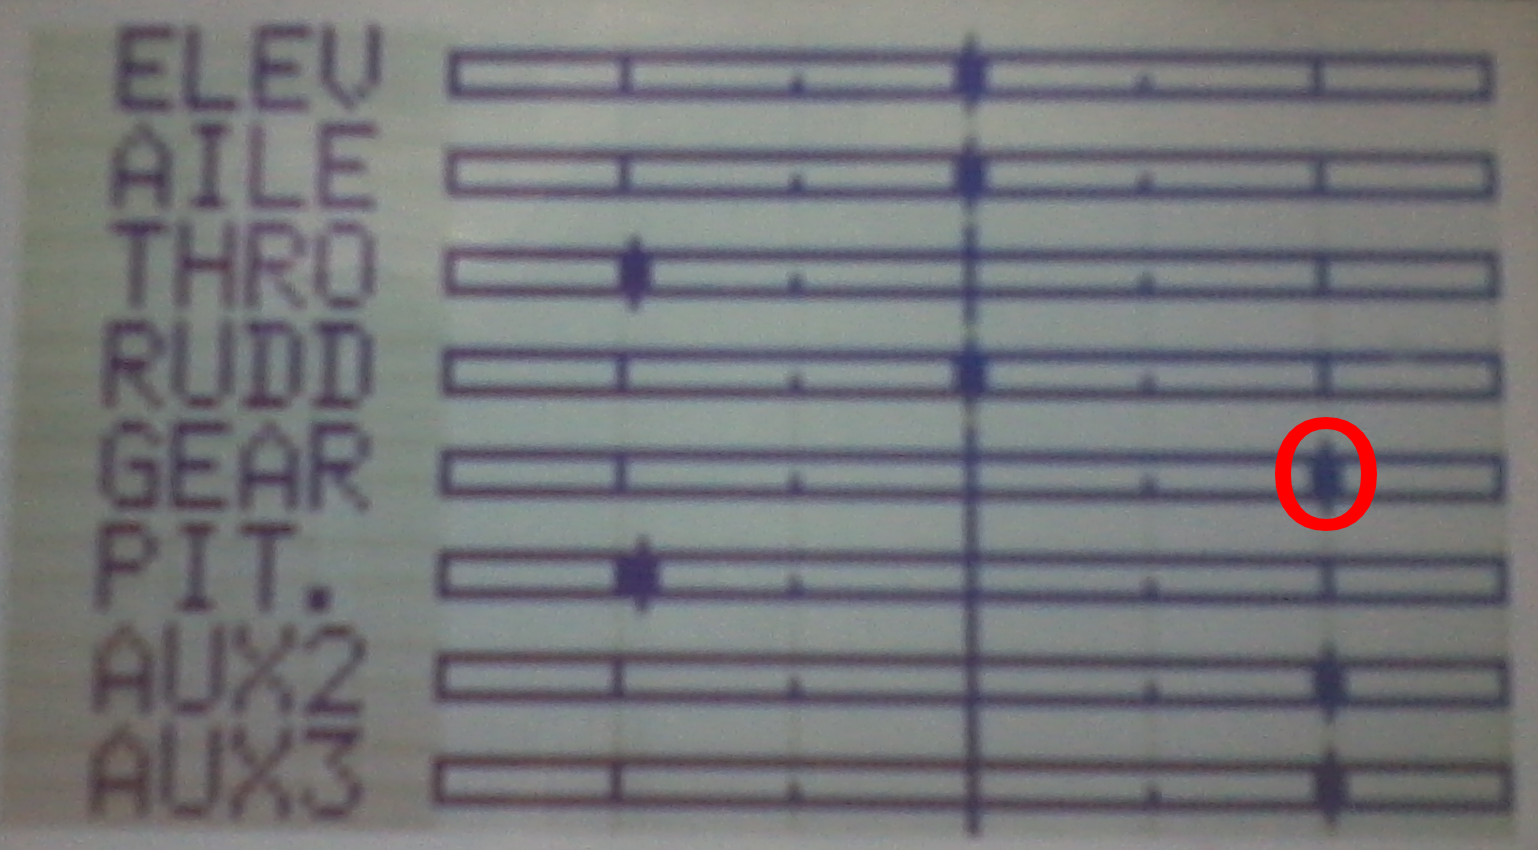
\includegraphics[width=0.7\textwidth]{./pics_switcheo/control_alto.png}
\caption{Monitor con GEAR alto}
\label{fig:control_alto}
\end{center}
\end{figure}

\section{Detección de la posición de la llave}

Para poder implementar el switcheo manual/automático será necesario poder detectar la posición de la llave. Esto es, debemos convertir la señal modulada proveniente del control en una señal binaria ON/OFF.\\
\\
Existen soluciones ya implementadas que se comercializan a muy bajo precio. De ellas, se seleccionó un circuito que se encarga de interpretar la señal y convertirla en una señal ON-OFF.\\
\\
A dicho circuito se le pueden conectar directamente las señales provenientes del receptor, ya que el mismo cuenta con la electrónica necesaria para interpretar dichas señales.\\
De esta forma, la salida del circuito será $Vcc(4.8V)$ si el tiempo en alto de la señal proveniente del receptor es mayor a $1.6ms$ y $GND (OV)$ si dicho tiempo es menor a $1.5ms$, lo cual se adapta perfectamente a nuestras necesidades.\\
\\
Es interesante, además, destacar que la placa adquirida es considerablemente pequeña, ya que la misma mide $1cm$ de lado y pesa apenas $0.3g$\\
\\
En la figura \ref{fig:circuito} puede apreciarse el circuito elegido.

\begin{figure}[H]
\begin{center}
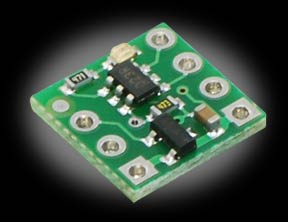
\includegraphics[width=0.7\textwidth]{./pics_switcheo/placa.jpg}
\caption{Circuito para interpretar la señal DCM}
\label{fig:circuito}
\end{center}
\end{figure}

Finalmente, introduciendo dicha señal a un multiplexor DSPT de dos canales, donde cada canal tiene un contacto normal abierto y otro normal cerrado, es posible realizar el switcheo en forma sencilla.\\
\\
En la figura \ref{fig:multiplexor} puede observarse el esquema de conexión de los componentes del sistema de switcheo.\\
\\
TODO: Hacer esquema de conexión.\\
\\
El multiplexor elegido es el $DG303AMIL$ de Vishay Electronics.

\end{document}